\documentclass[11pt]{exam}

\usepackage{amsmath, amssymb, multicol}
\usepackage{graphicx}
\usepackage{textcomp}
\usepackage{chessboard}
\usepackage{tikz}
\usepackage{adjustbox}
\usepackage{pdfpages}

\def\d{\displaystyle}
\def\b{\mathbf}
\def\R{\mathbf{R}}
\def\Z{\mathbf{Z}}
\def\st{~:~}
\def\bar{\overline}
\def\inv{^{-1}}
\def\r{2.5pt}
\def\v{circle (\r)}
\def\vo{node[circle, color=black, fill=white,  inner sep=2pt, minimum size = 17pt, draw]{}}

%\pointname{pts}
\pointsinmargin
\marginpointname{pts}
\addpoints
\pagestyle{head}
%\printanswers

\firstpageheader{Math 228}{\bf Coloring Graphs}{Wednesday, September 19}


\begin{document}

%space for name
%\noindent {\large\bf Name:} \underline{\hspace{2.5in}}
%\vskip 1em
% A \emph{proper vertex coloring} of a graph is a coloring in which no two adjacent vertices are colored the same color.  The \emph{chromatic number} of a graph is the smallest number of colors needed for a proper coloring of the graph.

\noindent\textbf{Instuctions}: For each graph on this and the next page:
\begin{itemize}
  \item Find a proper vertex coloring using some number of colors.
  \item State the chromatic number exactly, or at least give bounds for the chromatic number (what possible values could the chromatic number have?).
  \item Can you generalize?  Can you conclude anything about the chromatic number for particular sorts of graphs?
\end{itemize}


\begin{enumerate}
\begin{multicols}{2}
    \item\adjustbox{valign=m}{ 
        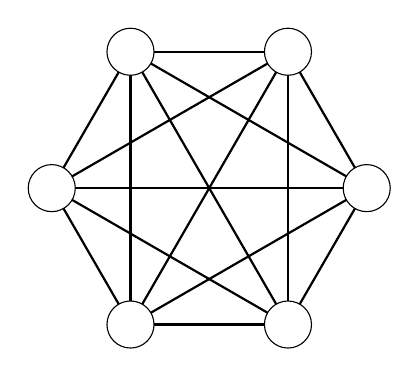
\begin{tikzpicture}[scale=2]
          \foreach \x in {0,...,5}{
          \coordinate (a\x) at (\x*60:1);
          }
          \foreach \x in {0,...,4}{
            \foreach \y in {\x,...,5}{
              \draw[thick] (a\x) -- (a\y);
            }
          \draw (a\x) \vo;
          }
          \draw (a5) \vo;
        \end{tikzpicture}
      }
      \columnbreak
    \item\adjustbox{valign=m}{
      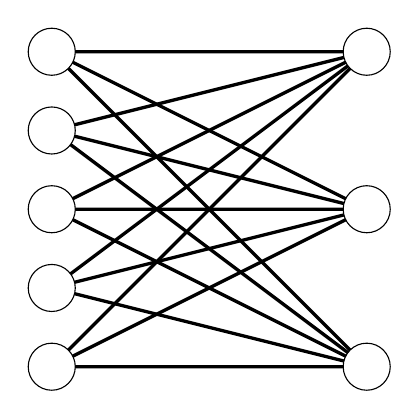
\begin{tikzpicture}[xscale=2]
        \foreach \x in {0,...,4}{
        \coordinate (l\x) at (0,\x);
        \coordinate (r\x) at (2,\x);
        }
        \foreach \x in {0,...,4}{
        \draw[very thick] (l\x) -- (r0) (l\x) -- (r2) (l\x) -- (r4);
        \draw (l\x) \vo;
        }
        \draw (r0) \vo (r2) \vo (r4) \vo;
      \end{tikzpicture}
      }
    \end{multicols}
    \vfill
    \begin{multicols}{2}
      \item\adjustbox{valign=m}{
      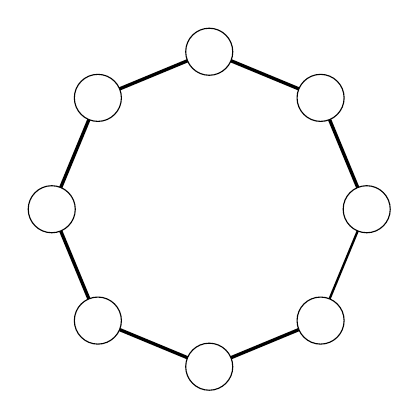
\begin{tikzpicture}
        \foreach \x in {0,...,7}{
        \coordinate (a\x) at (\x*360/8:2);
        }
        \draw[thick] (a7) -- (a0);
        \foreach \x in {0,...,6}{
          \pgfmathtruncatemacro{\next}{\x + 1}
          \draw[very thick] (a\x) -- (a\next);
          \draw (a\x) \vo;
        }
        \draw (a7) \vo;
      \end{tikzpicture}
      }
      \columnbreak
      \item\adjustbox{valign=m}{
      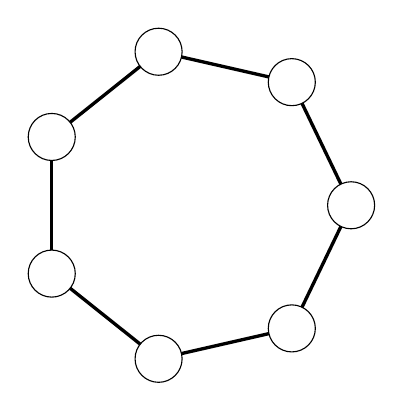
\begin{tikzpicture}
        \foreach \x in {0,...,6}{
        \coordinate (a\x) at (\x*360/7:2);
        }
        \draw[very thick] (a6) -- (a0);
        \foreach \x in {0,...,5}{
          \pgfmathtruncatemacro{\next}{\x + 1}
          \draw[very thick] (a\x) -- (a\next);
          \draw (a\x) \vo;
        }
        \draw (a6) \vo;
      \end{tikzpicture}
      }
    \end{multicols}
    \vfill
    \begin{multicols}{2}
      \item\adjustbox{valign=m}{
      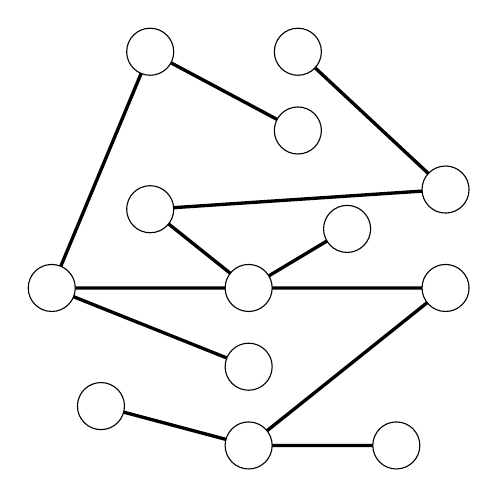
\begin{tikzpicture}[xscale=1.25]
        \coordinate (a) at (0,0);
        \coordinate (b) at (-2,0);
        \coordinate (c) at (2,0);
        \coordinate (d) at (0,-1);
        \coordinate (e) at (0,-2);
        \coordinate (f) at (-1.5,-1.5);
        \coordinate (g) at (-1,3);
        \coordinate (h) at (0.5,2);
        \coordinate (i) at (-1,1);
        \coordinate (j) at (1,.75);
        \coordinate (k) at (2,1.25);
        \coordinate (l) at (0.5,3);
        \coordinate (m) at (1.5,-2);
        \draw[very thick] (f) -- (e) -- (m) (e) -- (c) -- (a) -- (b) -- (d) (b) -- (g) -- (h) (a) -- (j) (a) -- (i) -- (k) -- (l);
        \foreach \x in {a,...,m}{
        \draw (\x) \vo;
        }
      \end{tikzpicture}
      }
      \columnbreak
      \item\adjustbox{valign=m}{
      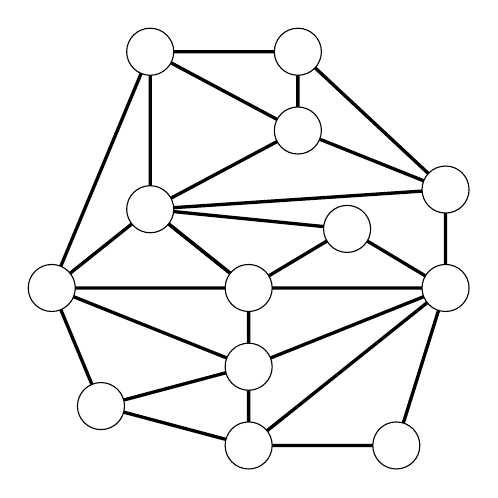
\begin{tikzpicture}[xscale=1.25]
        \coordinate (a) at (0,0);
        \coordinate (b) at (-2,0);
        \coordinate (c) at (2,0);
        \coordinate (d) at (0,-1);
        \coordinate (e) at (0,-2);
        \coordinate (f) at (-1.5,-1.5);
        \coordinate (g) at (-1,3);
        \coordinate (h) at (0.5,2);
        \coordinate (i) at (-1,1);
        \coordinate (j) at (1,.75);
        \coordinate (k) at (2,1.25);
        \coordinate (l) at (0.5,3);
        \coordinate (m) at (1.5,-2);
        \draw[very thick] (f) -- (e) -- (m) (e) -- (c) -- (a) -- (b) -- (d) (b) -- (g) -- (h) (a) -- (j) (a) -- (i) -- (k) -- (l);
        \draw[very thick] (a) -- (d) -- (c) -- (m) (d) -- (e) (d) -- (f) -- (b) -- (i) -- (g) -- (l) -- (h) -- (k) -- (c) -- (j) -- (i) -- (a) (i) -- (h);
        \foreach \x in {a,...,m}{
        \draw (\x) \vo;
        }
      \end{tikzpicture}
      }
    \end{multicols}
    \end{enumerate}



\end{document}
